\section{Experiments}

\begin{figure*}[t]
    \centering
    % \vspace{-5mm}
    \subfigure[Loss vs. epoch]{
    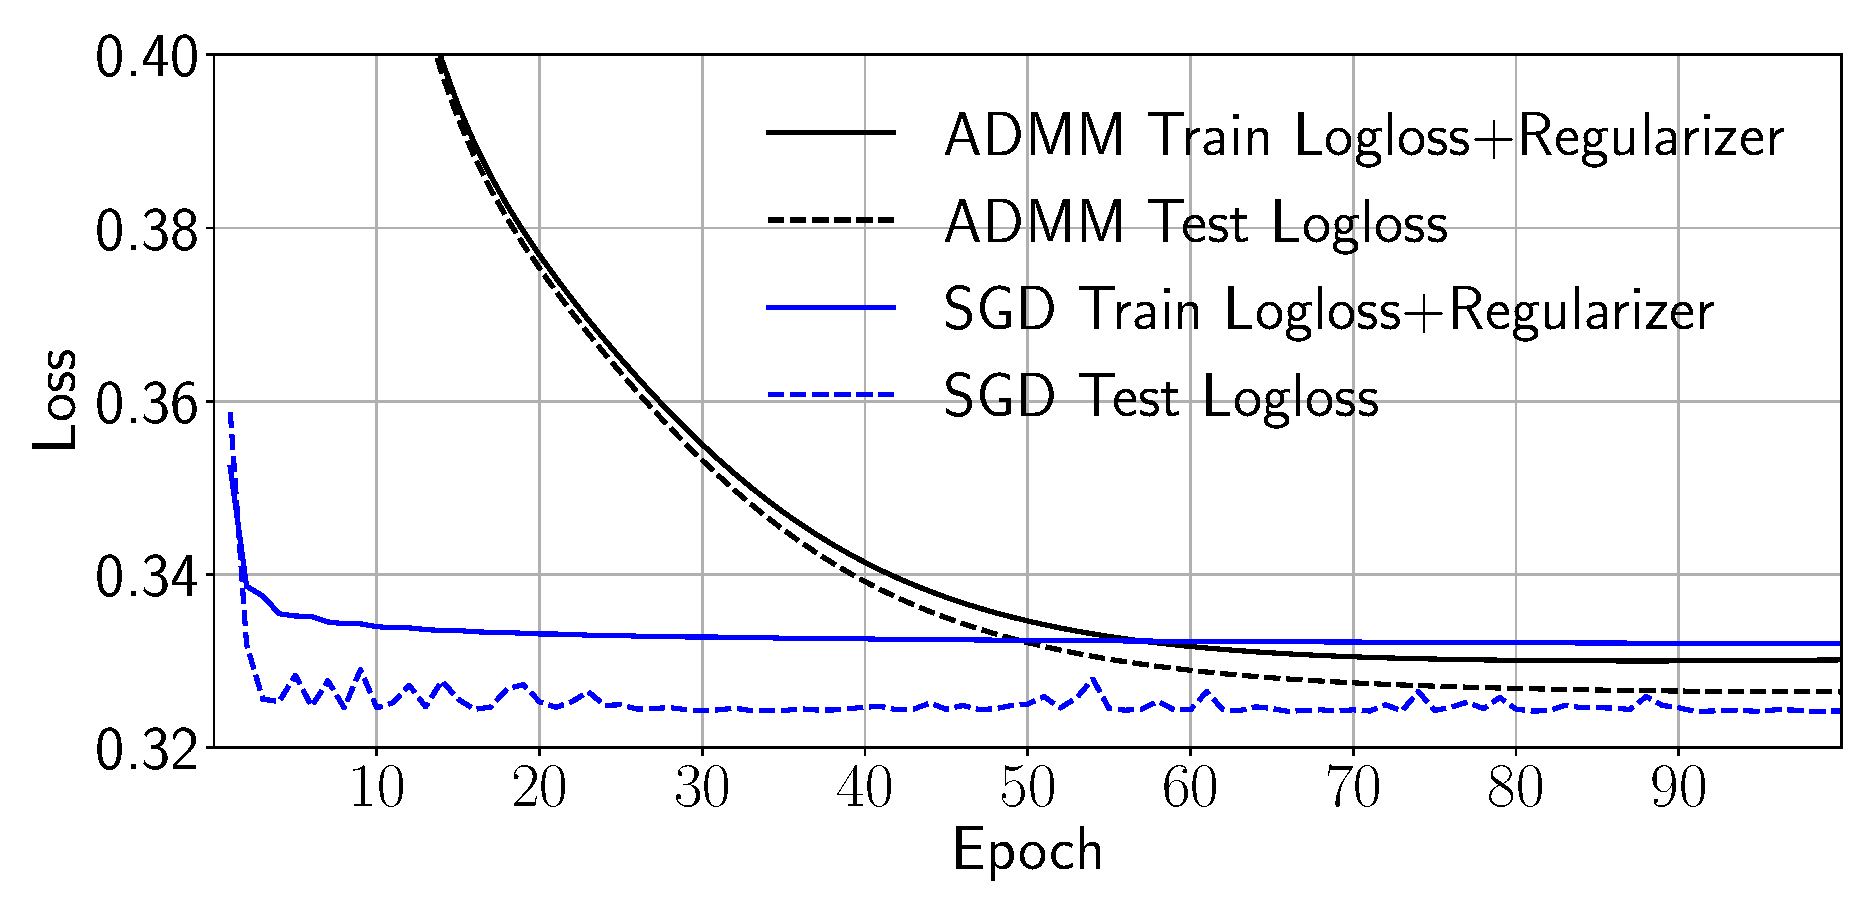
\includegraphics[width=3.4in]{figures/a9a_loss_vs_epoch}
    \label{fig:a9a_loss_vs_epoch}
    }
    % \hspace{-3.5mm}
    \subfigure[Test log loss under different noise levels]{
    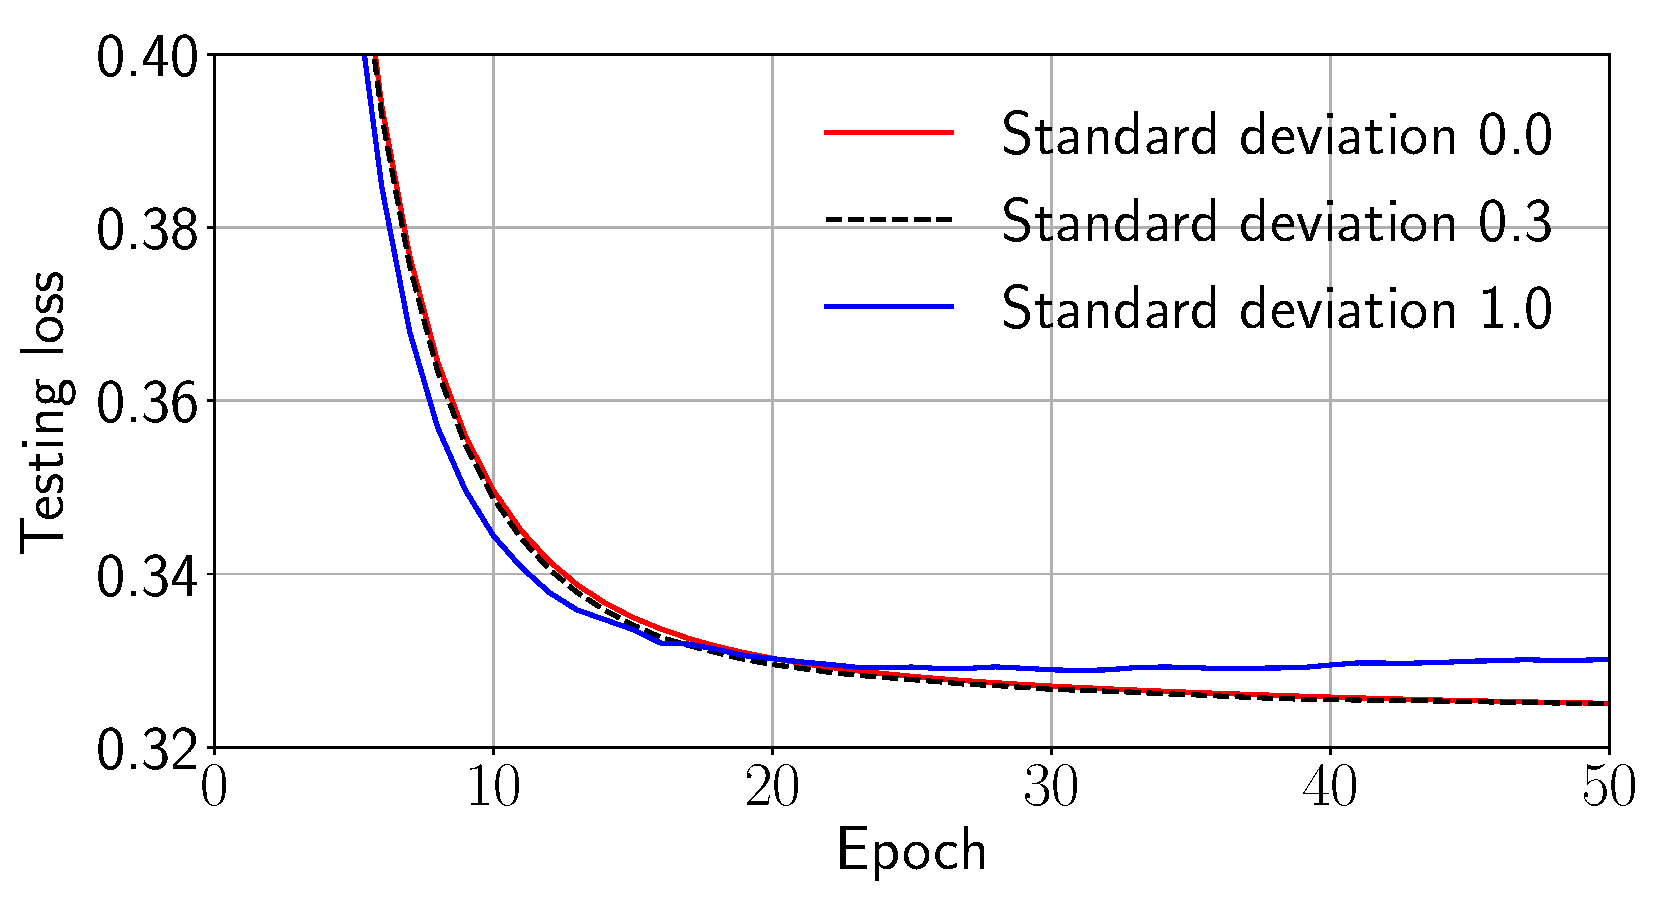
\includegraphics[width=3.4in]{figures/a9a_test_loss_vs_epoch_vary_noise}
    \label{fig:a9a_loss_vs_time}
    }
    % \vspace{-3.5mm}
    \caption{Performance over the \emph{a9a} data set with 32561 training samples, 16281 testing samples and 123 features.}
    \label{fig:a9a_train}
    \vspace{-4mm}
\end{figure*}

\begin{figure*}[t]
    \centering
    % \vspace{-5mm}
    \subfigure[Loss vs. epoch]{
    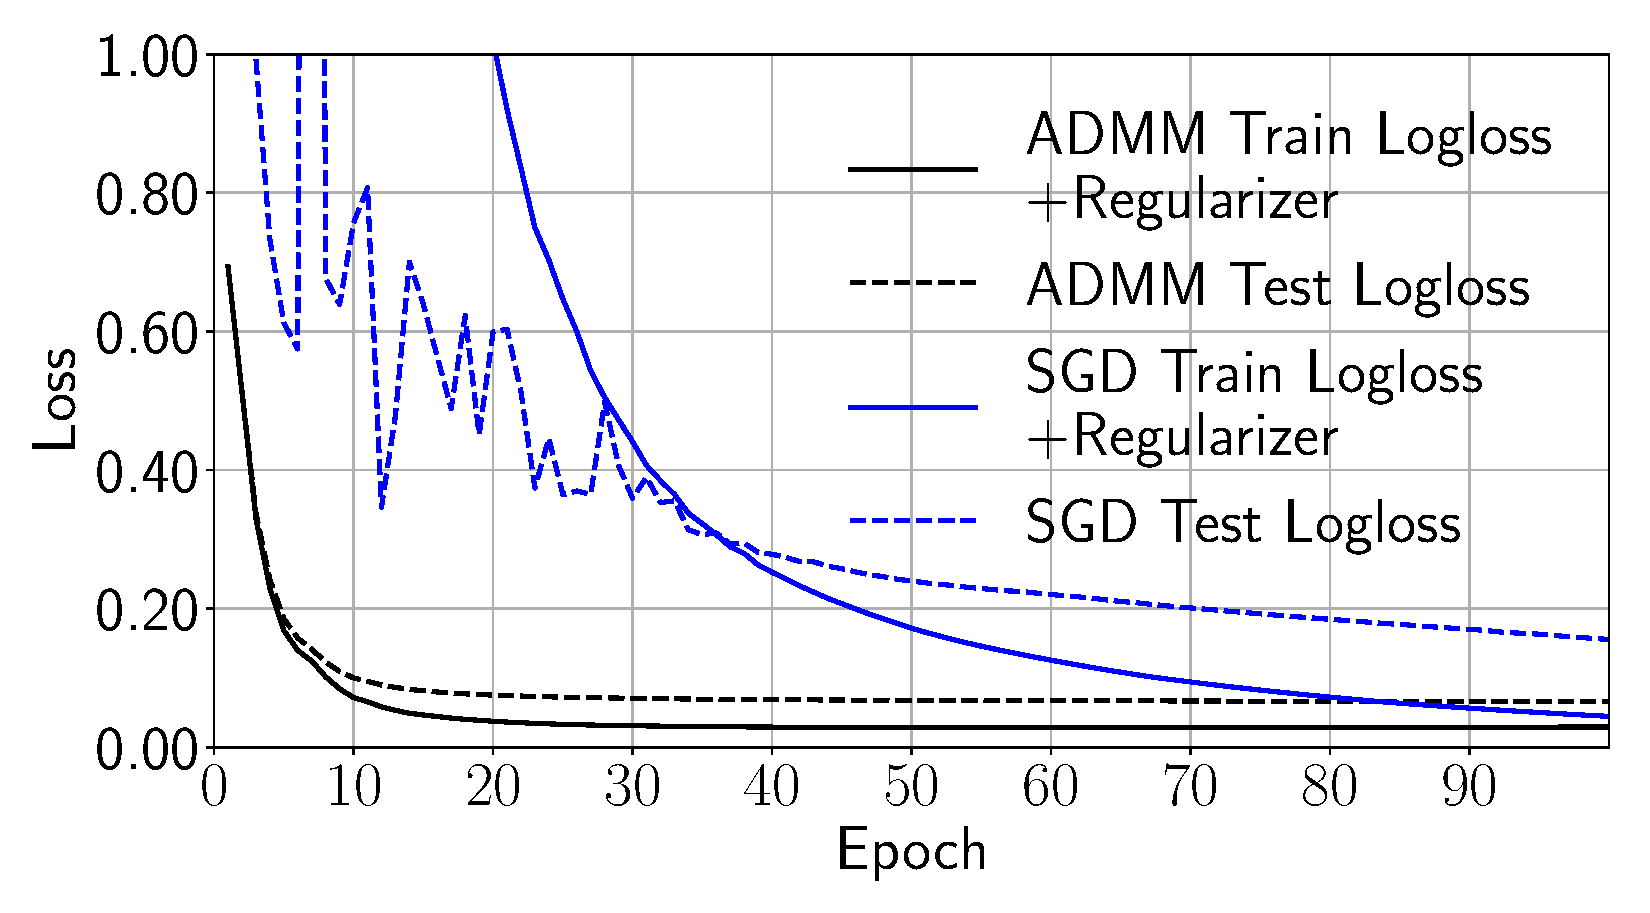
\includegraphics[width=3.4in]{figures/gisette_loss_vs_epoch}
    \label{fig:gisette_loss_vs_epoch}
    }
    % \hspace{-3.5mm}
    \subfigure[Test log loss under different noise levels]{
    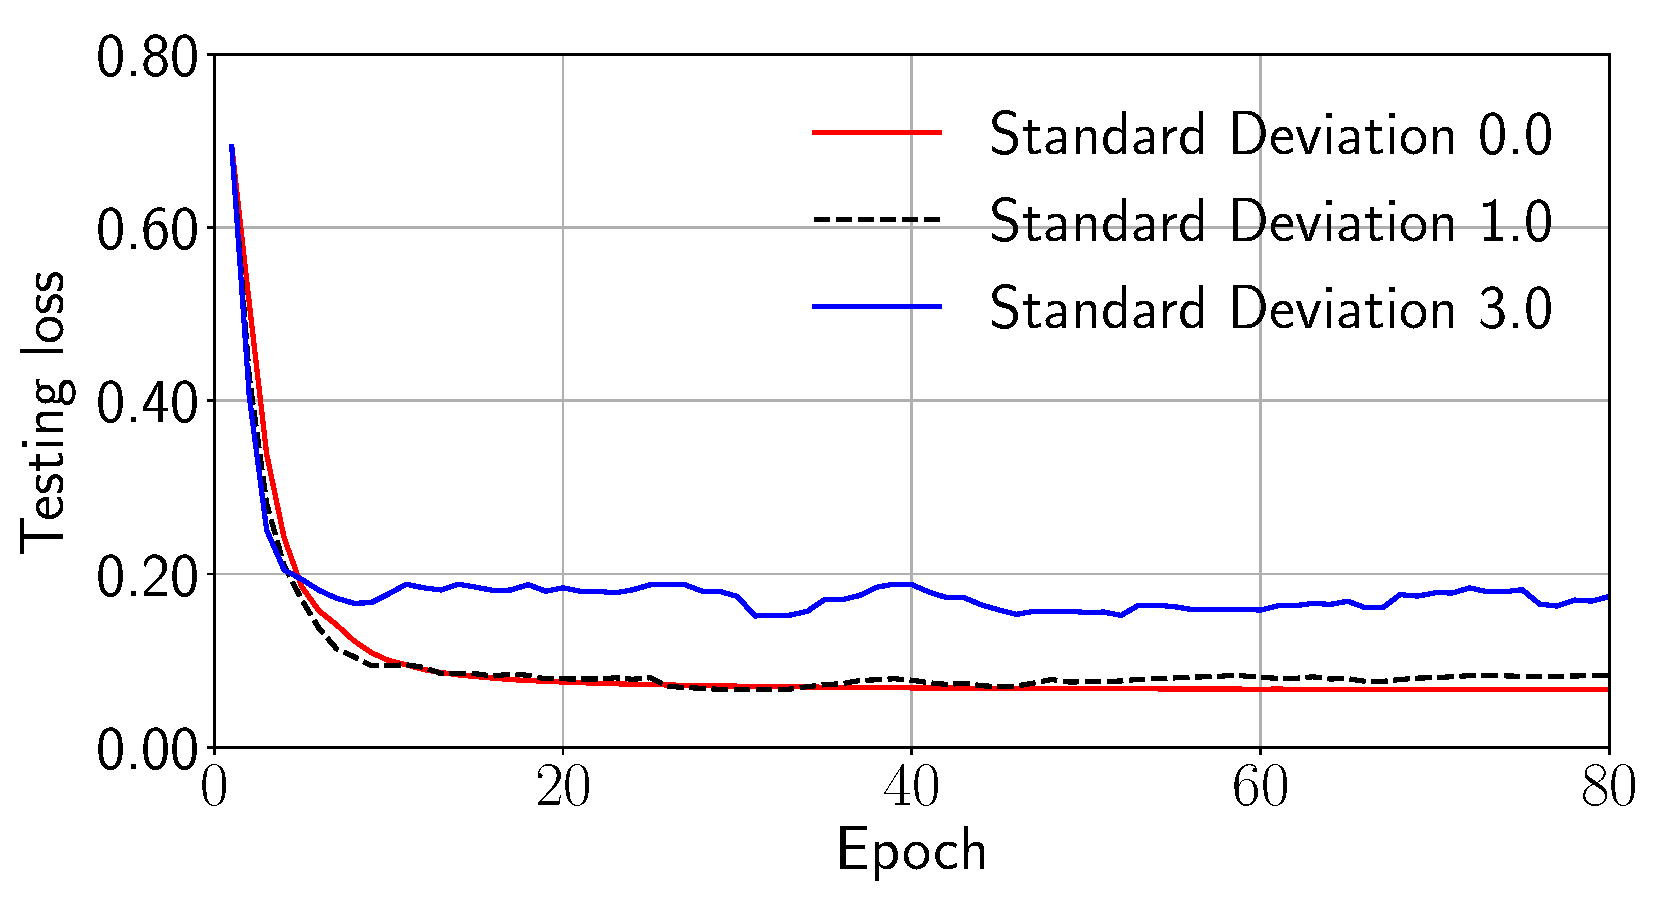
\includegraphics[width=3.4in]{figures/gisette_test_loss_vs_epoch_vary_noise}
    \label{fig:gisette_loss_vs_time}
    }
    % \vspace{-3.5mm}
    \caption{Performance over the \emph{gisette} data set with 6000 training samples, 1000 testing samples and 5000 features.}
    \label{fig:gisette_train}
    \vspace{-4mm}
\end{figure*}

\begin{figure*}[t]
    \centering
    % \vspace{-5mm}
    \subfigure[\emph{a9a} data set]{
    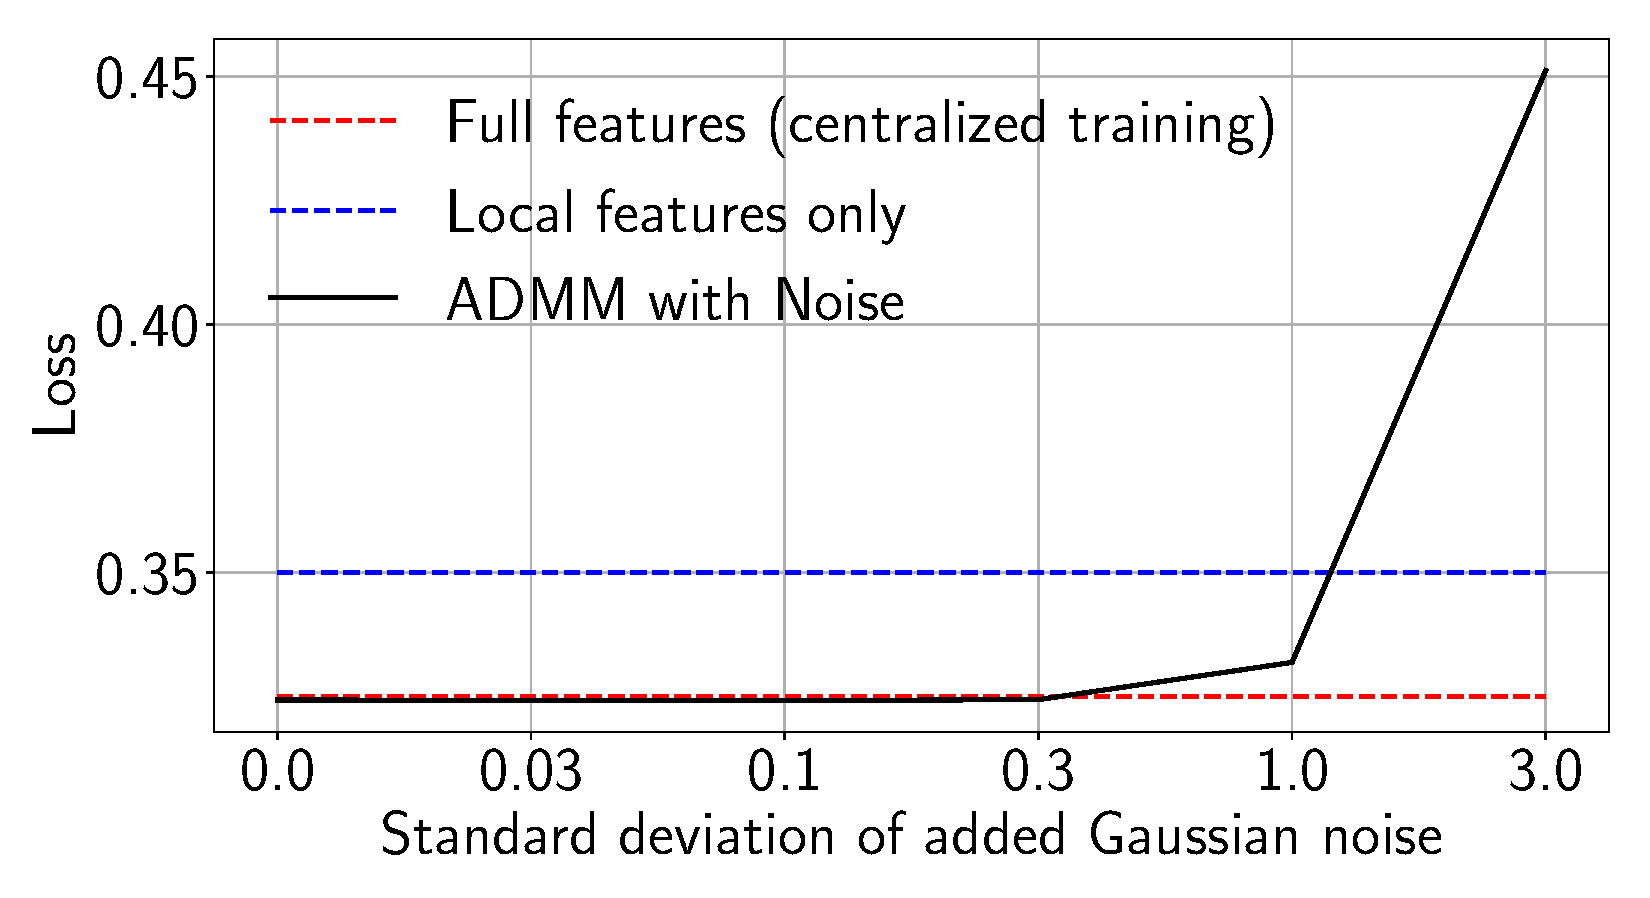
\includegraphics[width=3.4in]{figures/a9a_test_loss_vs_noise}
    \label{fig:a9a_test_loss_vs_noise}
    }
    % \hspace{-3.5mm}
    \subfigure[\emph{gisette} data set]{
    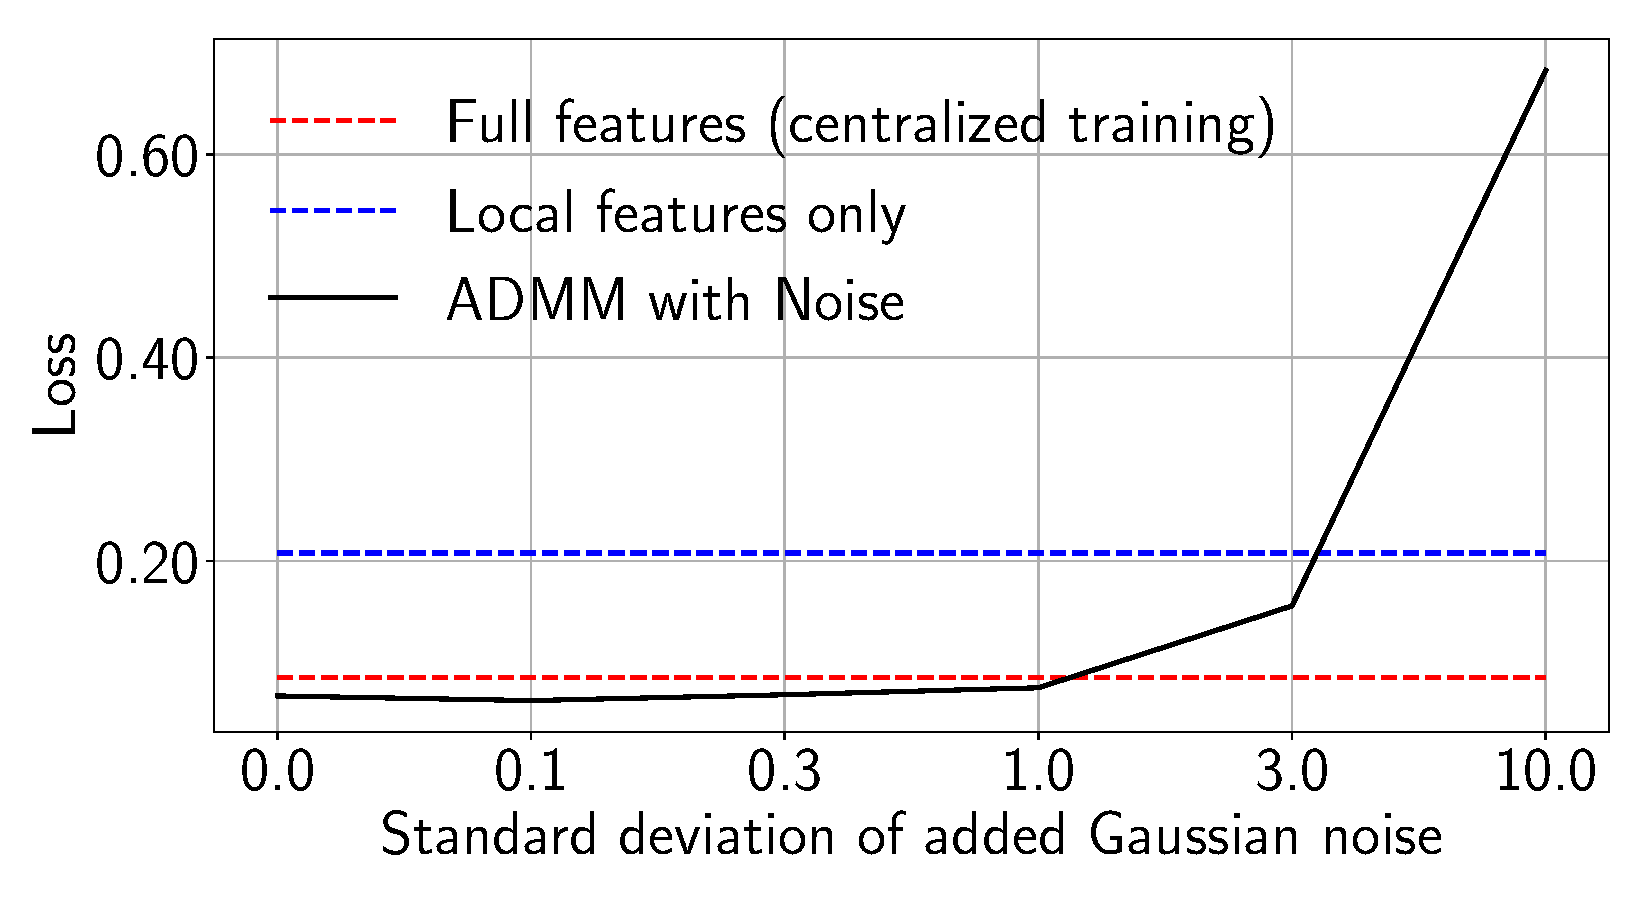
\includegraphics[width=3.4in]{figures/gisette_test_loss_vs_noise}
    \label{fig:gisette_test_loss_vs_noise}
    }
    % \vspace{-3.5mm}
    \caption{Test performance for ADMM under different levels of added noise.}
    \label{fig:loss_vs_noise}
     \vspace{-4mm}
\end{figure*}

We test our algorithm by training $l_2$-norm regularized logistic regression on two popular public datasets, namely, \emph{a9a} from UCI \cite{Dua:2019} and \emph{giette} \cite{guyon2005result}. We get the datasets from \cite{Liblinear:2019} so that we follow the same preprocessing procedure listed there. \emph{a9a} dataset is $4$ MB and contains 32561 training samples, 16281 testing samples and 123 features. We divide the dataset into two parts, with the first part containing the first 66 features and the second part remaining 57 features. The first part is regarded as the local party who wishes to improve its prediction model with the help of data from the other party. On the other hand, \emph{gisette} dataset is $297$ MB and contains 6000 training samples, 1000 testing samples and 5000 features. Similarly, we divide the features into 3 parts, the first 2000 features being the first part regarded as the local data, the next 2000 features being the second part, and the remaining 1000 as the third part. Note that \emph{a9a} is small in terms of the number of features and \emph{gisette} has a relatively higher dimensional feature space.

A prototype system is implemented in \emph{Python} to verify our proposed algorithm. Specifically, we use optimization library from \emph{scipy} to handle the optimization subproblems. We apply L-BFGS-B algorithm to do the $x$ update in \eqref{eq:pal_algo_x} and entry-wise optimization for $z$ in \eqref{eq:pal_algo_z}. We run the experiment on a machine equipped with Intel(R) Core(TM) i9-9900X CPU @ 3.50GHz and 128 GB of memory. 

We compare our algorithm against an SGD based algorithm proposed in \cite{hu2019fdml}.
We keep track of the training objective value (log loss plus the $l_2$ regularizer), the testing log loss for each epoch for different datasets and parameter settings. We also test our algorithm with different levels of Gaussian noise added. In the training procedure, we initialize the elements in $x$, $y$ and $z$ with $0$ while we initialize the parameter for the SGD-based algorithm with random numbers.

Fig.~\ref{fig:a9a_train} and Fig.~\ref{fig:gisette_train} show a typical trace of the training objective and testing log loss against epochs for \emph{a9a} and \emph{gisette}, respectively. On \emph{a9a}, the ADMM algorithm is slightly slower than the SGD based algorithm, while they reach the same testing log loss in the end. On \emph{gisette}, the SGD based algorithm converges slowly while the ADMM algorithm is efficient and robust. The testing log loss from the ADMM algorithm quickly converges to 0.08 after a few epochs, but the SGD based algorithm converges to only 0.1 with much more epochs. This shows that the ADMM algorithm is superior when the number of features is large.
In fact, for each epoch, the $x$ update is a trivial quadratic program and can be efficiently solved numerically. The $z$ update contains optimization over computationally expensive functions, but for each sample, it is always an optimization over a single scalar so that it can be solved efficiently via scalar optimization and scales with the number of features. 

Moreover, Corollary~\ref{theorem:overall_privacy} implies that the total differential privacy guarantee will be stronger if the number of epochs required for convergence is less. The fast convergence rate of the ADMM sharing algorithm also makes it more appealing to achieve differential privacy guarantees than SGD, especially in the case of wide features (\emph{gisette}).

Fig.~\ref{fig:loss_vs_noise} shows the testing loss for ADMM with different levels of Gaussian noise added. The other two baselines are the logistic regression model trained over all the features (in a centralized way) and that trained over only the local features in the first party. The baselines are trained with the built-in logistic regression function from \emph{sklearn} library. We can see that there is a significant performance boost if we employ more features to help training the model on Party 1. Interestingly, in Fig.~\ref{fig:gisette_test_loss_vs_noise}, the ADMM sharing has even better performance than the baseline trained with all features with \emph{sklearn}. It further shows that the ADMM sharing is better at datasets with a large number of features. 

Moreover, after applying moderate random perturbations, the proposed algorithm can still converge in a relatively small number of epochs, as Fig.~\ref{fig:a9a_loss_vs_time} and Fig.~\ref{fig:gisette_loss_vs_time} suggest, although too much noise may ruin the model.
%Thus, we can still achieve better performance than using local features only, although too much noise will ruin the model. 
Therefore, ADMM sharing algorithm under moderate perturbation can improve the local model and the privacy cost is well contained as the algorithm converges in a few epochs.


